%-------------------------------------------------------------------------------
% LATEX TEMPLATE ARTIKEL
%-------------------------------------------------------------------------------
% Dit template is voor gebruik door studenten van de de bacheloropleiding 
% Informatica van de Universiteit van Amsterdam.
% Voor informatie over schrijfvaardigheden, zie 
%                               https://practicumav.nl/schrijven/index.html
%
%-------------------------------------------------------------------------------
%	PACKAGES EN DOCUMENT CONFIGURATIE
%-------------------------------------------------------------------------------

\documentclass{uva-inf-article}
\usepackage[english]{babel}
\usepackage{tikz}
\usepackage{pdflscape}
\usepackage{todonotes}
\usepackage{listings}
\lstset{
basicstyle=\small\ttfamily,
columns=flexible,
breaklines=true
}

\usepackage[style=authoryear-comp]{biblatex}
\addbibresource{references.bib}

%-------------------------------------------------------------------------------
%	GEGEVENS VOOR IN DE TITEL, HEADER EN FOOTER
%-------------------------------------------------------------------------------

% Geef je artikel een logische titel die de inhoud dekt.
\title{Shogun Post Documentation}

% Vul de naam van de opdracht in zoals gegeven door de docent en het type 
% opdracht, bijvoorbeeld 'technisch rapport' of 'essay'.
% \assignment{}
% \assignmenttype{}

% Vul de volledige namen van alle auteurs in en de corresponderende UvAnetID's.
\authors{Jari Andersen}
% \uvanetids{}

% Vul de naam van je tutor, begeleider (mentor), of docent / vakcoördinator in.
% Vermeld in ieder geval de naam van diegene die het artikel nakijkt!
% \tutor{}
% \mentor{}
% \docent{}

% Vul hier de naam van je tutorgroep, werkgroep, of practicumgroep in.
% \group{SignLab, VisualisationLab}

% Vul de naam van de cursus in en de cursuscode, te vinden op o.a. DataNose.
% \course{}
% \courseid{}

% Dit is de datum die op het document komt te staan. Standaard is dat vandaag.
\date{\today}

%-------------------------------------------------------------------------------
%	VOORPAGINA 
%-------------------------------------------------------------------------------

\begin{document}
\maketitle

%-------------------------------------------------------------------------------
%	INHOUDSOPGAVE EN ABSTRACT
%-------------------------------------------------------------------------------
% Niet toevoegen bij een kort artikel, zeg minder dan 10 pagina's!

%TC:ignore
\tableofcontents
%\begin{abstract}
%\end{abstract}
%TC:endignore
\newpage
%-------------------------------------------------------------------------------
%	INHOUD
%-------------------------------------------------------------------------------
% Hanteer bij benadering IMRAD: Introduction, Method, Results, Discussion.
\section{Introduction}
Welcome to the Shogun Post Documentation! In this guide, we delve into various tools and skills within Shogun Post, designed to streamline your post-production workflows effectively. Throughout this documentation, we'll address crucial aspects such as identifying and resolving bugs, as well as highlighting best practices to optimize your post-production processes. Additionally, we'll delve into scripting techniques and the creation of efficient export pipelines, empowering you to automate tasks and enhance productivity.
Our exploration extends to a range of indispensable tools, including retargeting mechanisms, strategies for rectifying marker issues, and integration techniques for importing StretchSense data.

\section{Best practices and tips}

\subsection{Creating scripts}
Creating Scripts in Shogun Post can be done through their script editor. Here are some more tips on them:
\begin{itemize}
    \item Use scripts by Vicon from the script folder to get an idea on how to write them.
    \item Use the record function in Shogun Post's script editor to record your clicks and actions in the software (see Figure \ref{fig:recordButton}). This will make finding certain functionalities and scripting quickly much easier.
    \item If you want to reuse scripts, make buttons for them by right clicking somewhere in the upper tab. You can also create new tabs for buttons.
\end{itemize}

\begin{figure}[hbt!]
    \centering
    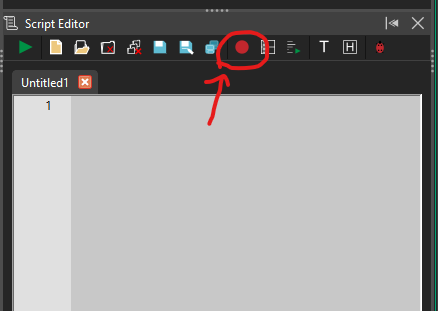
\includegraphics[]{imgs/recordButton.png}
    \caption{Location of the scripting record button in Shogun Post.}
    \label{fig:recordButton}
\end{figure}


\subsection{Export pipelines}
Often, when recording many takes, we want to export each of them out of Shogun Post in the same manner. For this, we can use the ``Batching" functionalities (see Figure \ref{fig:batching}). In the Batching tab, we can select which files we want to export, and define where and how they should be exported. 
\begin{figure}[hbt!]
    \centering
    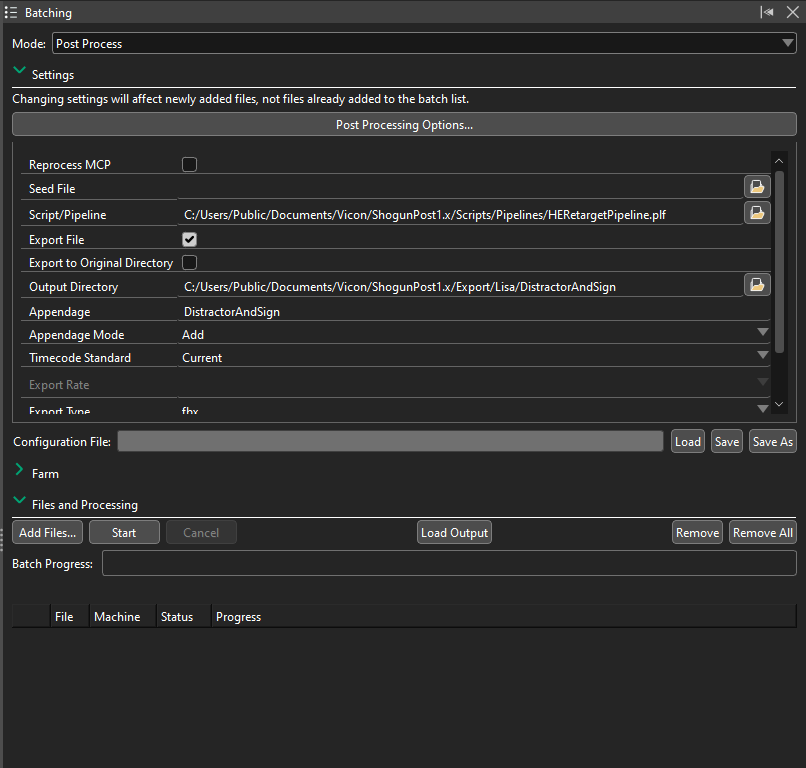
\includegraphics[width=\textwidth]{imgs/Batching.png}
    \caption{The batching tab in Shogun Post.}
    \label{fig:batching}
\end{figure}

These functionalities however, are not always enough. For example, if we want to remove the ``wand" prop from every take, we would not be able to do this with the default functionalities. To this end, we can create pipeline scripts (extension ``.plf"). In the pipeline scripts we can define what operations (hsl or py scripts) to run before exporting a take. See Figure \ref{fig:pipelineHE} for an example pipeline that sets a frame rate, imports StretchSense FBX files and retargets before exporting.
\begin{figure}[hbt!]
    \centering
    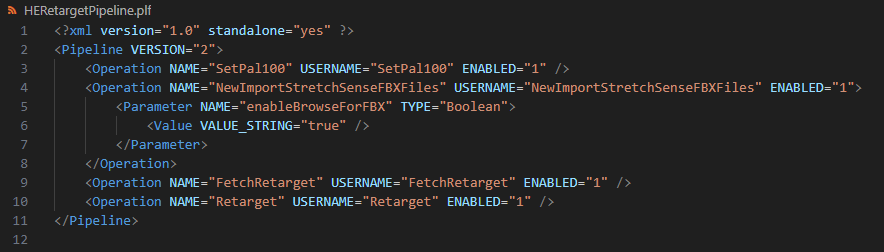
\includegraphics[width=\textwidth]{imgs/pipelineHE.png}
    \caption{An example pipeline script where we want to set the frame rate to PAL100, import StretchSense fbx files, and retarget before exporting.}
    \label{fig:pipelineHE}
\end{figure}

\subsection{Retargeting}
\todo{Process in short, tips on hands}

\subsection{Combining Vicon and StretchSense data}
\todo{best practices for aligning}


\section{Bugs and fixes}
In this section we go over various bugs we found and fixes to solve them.

\subsection{Unreal import bug}
\begin{figure}[hbt!]
    \centering
    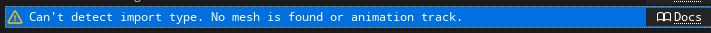
\includegraphics[width=\textwidth]{imgs/UEImportBug.png}
    \caption{Unreal import bug.}
    \label{fig:importBugUE}
\end{figure}
When importing a retarget into Unreal Engine, we came acros the following bug: ``Can't detect import type. No mesh is found or animation track". In Shogun Post everything seems to be working, the retargeted animation is displayed and we selected the retarget branch for export. No errors occured on Shogun Post end, however, the bug is due to Shogun Post. After importing the retargeted FBX animations into Blender, we can view the skeleton, but the animation itself is not present. In our case, the bug occurred because we altered the frame rate after retargeting. To fix this, simply retarget over the playrange again and export like usual. I believe the displayed animation appears correct after altering the frame rate because it is consistently interpolated between frames.


%-------------------------------------------------------------------------------
%	REFERENTIES
%-------------------------------------------------------------------------------

\printbibliography

%-------------------------------------------------------------------------------
%	BIJLAGEN 
%-------------------------------------------------------------------------------

%TC:ignore
% \appendix 
% \section{Bijlage {\LaTeX} code}
% Bijgevoegd zijn de \textattachfile{main.tex}{code} en 
% \textattachfile{references.bib}{bibliografie}.
%TC:endignore

%-------------------------------------------------------------------------------
\end{document}